\section*{Propagazione del segnale nell'aria}
La propagazione del segnale nell'atmosfera può essere classificata in base alle bande di frequenza e alle relative caratteristiche. Di seguito vengono elencate le diverse bande di classificazione, le iniziali, i range di frequenza e le principali caratteristiche:
\begin{table}[h!]
\centering
\begin{tabular}{llll}
\hline
\textbf{Classification Band} & \textbf{Initials} & \textbf{Frequency Range} & \textbf{Characteristics} \\
\hline
Extremely low frequency & ELF & $<$ 300 Hz & Ground wave \\
Very low frequency & VLF & 3 kHz - 30 kHz & Ground/Sky wave \\
Low frequency & LF & 30 kHz - 300 kHz & Ground/Sky wave \\
Medium frequency & MF & 300 kHz - 3 MHz & Ground/Sky wave \\
High frequency & HF & 3 MHz - 30 MHz & Sky wave \\
Very high frequency & VHF & 30 MHz - 300 MHz & Space wave \\
Ultra high frequency & UHF & 300 MHz - 3 GHz & Space wave \\
Super high frequency & SHF & 3 GHz - 30 GHz & Space wave \\
\hline
\end{tabular}
\end{table}


Dalla frequenza delle onde, da cui dipende la modalità di propagazione attraverso il canale, si indentificano i seguenti meccanismi di propagazione:

\begin{itemize}
    \item \textbf{Ground wave} (fino a 2 MHz): le onde si propagano seguendo la curvatura terrestre riuscendo a raggiungere un ricevitore oltre l'orizzonte, in certi casi anche a centinaia di chilometri di distanza.
    \item \textbf{Sky wave} (1-10 MHz): le onde sono riflesse dalla ionosfera e si propagano rimbalzando tra quest'ultima e la superficie terrestre, riuscendo a coprire distanze nell'ordine dei migliaia di chilometri.
    \item \textbf{Space wave} (da 30 MHZ): le onde richiedono un line-of-sight per poter essere ricevute correttamente, inoltre bisogna tenere in considerazione che maggiore è la frequenza maggiore sarà l'attenuazione. Il ricevitore oltre alla componente diretta riceve anche componenti aggiuntive, date dalla riflessione delle onde su ostacoli lungo il percorso.
\end{itemize}



Le space wave rappresentano il meccanismo più importante dato che la maggior parte dei sistemi di comunicazione ne fa affidamento. Le space wave sono soggette a diversi fenomeni di propagazione:
\begin{itemize}
    \item \textbf{Riflessione}: quando il segnale impatta con un oggetto liscio molto grande rispetto alla lunghezza d'onda può essere riflesso, ovvero rimbalza e prosegue con angolo differente, oppure passa attraverso.
    \begin{center}
        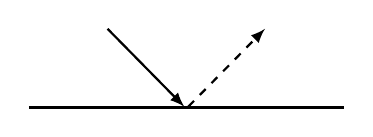
\begin{tikzpicture}
            \draw[thick] (-2,0) -- (2,0);
            \draw[thick, -latex] (-1,1) -- (-0.025,0.01);
            \draw[thick, -latex, dashed] (0.025,0.01) -- (1,1);
        \end{tikzpicture}
    \end{center}



    
   
    \item \textbf{Diffrazione}: quando il segnale è ostruito da oggetti con superfici taglienti, parte del segnale può modificare l'angolo con cui si propaga. Questo fenomeno permette in certe condizioni di ricevere un segnale anche in assenza di un line-of-sight a causa di un oggetto che crea una zona d'ombra, ovviamente l'energia ricevuta sarà minore rispetto a quella originaria del segnale.
    \begin{center}
        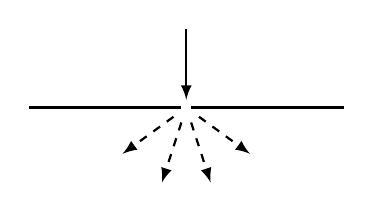
\begin{tikzpicture}
            \draw[thick] (-2,0) -- (-0.0625,0);
            \draw[thick] (0.0625,0) -- (2,0);
            \draw[thick, -latex] (0,1) -- (0,0.1);
           
            \draw[thick, -latex, dashed] (-0.1618033988749895, -0.1175570504584946) -- (-0.8090169943749476, -0.587785252292473);
            \draw[thick, -latex, dashed] (-0.061803398874989514, -0.1902113032590307) -- (-0.30901699437494756, -0.9510565162951535);
            \draw[thick, -latex, dashed] (0.061803398874989444, -0.19021130325903074) -- (0.30901699437494723, -0.9510565162951536);
            \draw[thick, -latex, dashed] (0.16180339887498946, -0.11755705045849467) -- (0.8090169943749473, -0.5877852522924734);
        \end{tikzpicture}
    \end{center}


    
    \item \textbf{Scattering}: quando il segnale impatta con oggetti di piccola dimensione rispetto alla lunghezza d'onda si ha una propagazione in più direzioni del segnale.
    \begin{center}
        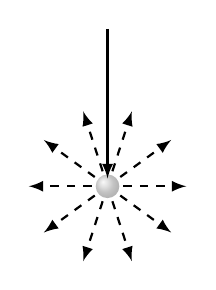
\begin{tikzpicture}
            \shade[ball color=black!40, opacity=0.4] (0,0) circle (0.15cm);
            \draw[thick, -latex] (0,2) -- (0,0.1);
            \draw[thick, -latex, dashed] (0.16180339887498948, 0.11755705045849463) -- (0.8090169943749475, 0.5877852522924731);
            \draw[thick, -latex, dashed] (0.06180339887498949, 0.1902113032590307) -- (0.30901699437494745, 0.9510565162951535);
            \draw[thick, -latex, dashed] (-0.061803398874989465, 0.19021130325903074) -- (-0.30901699437494734, 0.9510565162951536);
            \draw[thick, -latex, dashed] (-0.16180339887498946, 0.11755705045849466) -- (-0.8090169943749473, 0.5877852522924732);
            \draw[thick, -latex, dashed] (-0.2, 2.4492935982947065e-17) -- (-1.0, 1.2246467991473532e-16);
            \draw[thick, -latex, dashed] (-0.1618033988749895, -0.1175570504584946) -- (-0.8090169943749476, -0.587785252292473);
            \draw[thick, -latex, dashed] (-0.061803398874989514, -0.1902113032590307) -- (-0.30901699437494756, -0.9510565162951535);
            \draw[thick, -latex, dashed] (0.061803398874989444, -0.19021130325903074) -- (0.30901699437494723, -0.9510565162951536);
            \draw[thick, -latex, dashed] (0.16180339887498946, -0.11755705045849467) -- (0.8090169943749473, -0.5877852522924734);
            \draw[thick, -latex, dashed] (0.2, -4.898587196589413e-17) -- (1.0, -2.4492935982947064e-16);
        \end{tikzpicture}
    \end{center}
 





    \item \textbf{Assorbimento e rifrazione}: si tratta di fenomeni meno importanti, ma che comunque possono modificare la propagazione del segnale. 
\end{itemize}

Gli effetti generati da questi fenomeni possono essere riassunti in due diversi tipi di attenuazione del segnale:
\begin{itemize}
    \item \textbf{Small-scale fading}: modella fluttazioni rapide della potenza del segnale su lunghezze paragonabili a quella dell'onda.
    \item \textbf{Large-scale fading}: modella la variazione della potenza del segnale su lunghe distanze.
\end{itemize}


\subsection*{Large-scale fading}
Il LSF modella la variazione della potenza del segnale in base alla fistanza fra trasmettitore e ricevitore, tipicamente variando per distanze nell'ordine del metro. Gli effetti sono modellati attraverso la combinazione di path loss e shadowing:
Il path loss rappresenza un'approssimazione delle equazioni di Maxwell.
\begin{equation}
    P_{RX} \approx P_{TX} \cdot \Gamma(f_0, d_0) \cdot \left( \frac{d_0}{d} \right)^n \quad \text{for } d > d_0
\end{equation}

dove \( \Gamma(f_0, d_0) \approx \left( \frac{\lambda}{4 \pi d_0} \right)^2 \) rappresenta il termine di campo vicino, \( P_{TX} \) è la potenza trasmessa, \( d_0 \) è la distanza di riferimento e \( n \) è l'esponente del path loss. Quest'ultimo dipende dall'ambiente in cui ci si trova, ad esempio in un ambiente urbano il valore di \( n \) varia tra 2.7 e 3.5.



La formula, deterministica, che fornisce il valore di attenuazione dato dal path loss è:
\[
    A_{PL} = \frac{P_{TX}}{P_{RX}} = \Gamma(f_0, d_0) \cdot \left( \frac{d_0}{d} \right)^n
    A_{PL}^{dB} = 10 \cdot \log_{10}(A_{PL}) = \Gamma(f_0, d_0)_{dB} + n \cdot 10 \cdot \log_{10}(d_0) - n \cdot 10 \cdot \log_{10}(d)
\]


Nel vuoto l'attenuazione del segnale in base alla distanza è data dalla relazione
\[
    P_{RX} = P_{TX} \cdot \frac{A}{4\pi d^2}  
\]
dove \( A \) è l'area dell'antenna in ricezione, che tipicamente è \( A = \lambda^2 \) dove \( \lambda \) è la lunghezza d'onda del segnale.


Per frequenze inferiori ai 6GhZ l'attenuazione dipende dalle frequenze con una relazione quadratica, tuttavia oltre tale scoglio la lunghezza d'onda è sufficientemente piccola per interagire con molecole presenti nell'aria, in particulare ossigeno e vapore acqueo, incrementando ulteriormente l'attenuazione.

Nella progettazione di sistemi di comunicazione wireless è essenziale tenere in considerazione il rapportarto tra frequenza utilizzata e distanza copribile da una singola antenna.

\subsection*{Shadowing}

Dati due punti alla stessa distanza dal trasmettitore se si considerasse unicamente il path loss avrebbe la stessa attenuazione, tuttavia nella realtà vi è una componente aleatoria da dover considerare, modellabile tramite shadowing. La componente aleatoria è dovuta alla presenza di ostacoli differenti che coprono parzialmente il segnale ricevuto. La componente aleatoria è caratterizzata da una distribuzione log-normale con parametri $\mu = 0$ e $\sigma_S$, espressi in dB, quindi una distribuzione normale con parametri espressi in dB.
\begin{equation}
    p(A_S) = \frac{1}{\sqrt{2\pi \sigma_S}} e^{-\frac{A_S^2}{2\sigma_S^2}}
\end{equation}




Gli effetti del path loss e dello shadowing sono sommati per ottenere le variazioni dovute al large scale fading. 
\[
    A_{LS} = A_{PL} \cdot A_S \quad \text{scala lineare}
\]

\[
    A_{LS}^{dB} = A_{PL}^{dB} + A_S^{dB} \quad \text{scala logaritmica}
\]


PL è deterministico e dipende dall'esponente scelto in base all'ambiente circostante e dalla distanza tra trasmettitore e ricevitore, mentre shadowing aleatorio e distribuito come una log-normale. Entrambi gli eggetti contribuisoono a variazioni nella potenza media ricevuta, le cui fluttuazioni sono significative solo per grandi distanze, considerando la lughezza d'onda.



\section*{Small scale fading}

SSF modella le variazioni aleatorie della potenza istantanea su sistanze nell'ordine della lunghezza d'onda, dovute ai vari fenomeni di propagazione delle onde che determinano la ricezione di repliche del segnale, ognuno con un certo ritardo, fase ed attenuazione. Il canale di tramissione è modellato come un filtro LTI, la cui risposta impulsiva dipende dagli effetti SSF.

\[
    h(t) = A_{LS} \sum_{\ell=0}^{N_c-1} \alpha_{\ell} e^{j\phi_{\ell}} \delta(t - \tau_{\ell})
\]

Dove \( A_{LS} \) è l'attenuazione dovuta al large scale fading, \( \alpha_{\ell} \) e \( \phi_{\ell} \) sono rispettivamente ampiezza e fase del segnale \(\ell\)-esimo, e \( \tau_{\ell} \) è il ritardo temporale. La risposta impulsiva del canale è la somma delle risposte impulsiva di ogni singolo percorso.

Per quanto riguarda i parametri delle varie repliche:
\begin{itemize}
    \item \textbf{Attenuazione} ($\alpha_\ell$): sono modellati come variabili aleatorie, tipicamente con distribuzione di Rayleigh, derivante dal fatto che le componenti in gase e quadratura hanno una distribuzione normale.
    \[
        \alpha e^{j\phi_i} = x_i + j y_i \quad \text{con } x_i, y_i \sim \mathcal{N}(0, \sigma^2)
    \]
    \[
        \|\alpha e^{j\phi_i}\| = \sqrt{x_i^2 + y_i^2} \sim \text{Rayleigh}(\sigma)
    \]
    \item \textbf{Fase} ($\phi_\ell$): sono modellati come variabili distribuite uniformemente nell'intervallo $[0, 2\pi]$.
\end{itemize}

La ricezione di più repliche, soprattutto se notevolemnte distanziate tra loro, genera ISI.
\[
    x(t) = \sum_{i} c_i g(t - iT) \quad \text{uscita filtro in ricezione (senza rumore)}
\]
\[
    g(t) = g_T(t) \ast h(t) \ ast g_R(t) = g_H(t) \ast h(t) = \sum_{\ell=0}^{N_c-1} \alpha_{\ell} e^{j\phi_{\ell}} g_H(t - \tau_{\ell})
\]

\[
  x(m) = \sum_{k}  C_{m-k}g(k) = c_m g(0) + \underbrace{\sum_{k \neq 0} c_{m-k} g(k)}_{\text{ISI}}
\]

\[
    g(k) = \sum_{\ell=0}^{N_c-1} \alpha_{\ell} e^{j\phi_{\ell}} g_H(k - \tau_{\ell})
\]

Sebbene quindi si scelga un filtro che rispetti la condizione di Nyquist, gli effetti del canale non permettono di rimuovere completamente l'ISI, generata dal fatto che g(k) non si annulla.


Il delay spread permette di misurare la dispersione temporale introdotta dal canale:
\begin{itemize}
    \item $\sigma_\tau \ll T$: delay spread inferiore al symbol time, il canale è detto \textbf{flat fading}  e l'effetto dell'ISI è trascurabile in quanto le varie repliche ricevute fanno tutte riferimento allo stesso simbolo.
    \item $\sigma_\tau > T$: delay spread maggiore del symbol time, il canale è detto \textbf{multipath} e l'effetto dell'ISI non è più trascurabile in quanto le varie repliche, appartenti a simboli differenti, interferiscono tra loro.
\end{itemize}

In entrambi i casi il canale è detto \textbf{multipath} in quanto la ricezione del segnale avviene attraverso più replichem poi si aggiunge una classificazione ulteriore dovuta al delay spread.
flat fading. La coerenza temporale è il tempo entro il quale il canale è circa costante.
\[
    B_c \approx \frac{1}{5\sigma_\tau}
\]
Se $B_c > B_S \approx \frac{1}{T}$, ovvero la banda del segnale trasmesso, non si avrà alcune distorsione, il canale risulta \textbf{flat fading}. In caso contrario, se $B_c < B_S$ il canale è detto \textbf{frequency selective}. 

La coherence bandwidth può essere determinata considerando la densità spettrale di potenza.
I delay sono modellabili come variabili aleatorie $\tau$, perché per ottenere proprietà statistiche si possono applicare le operazioni standard per il calcolo del valor medio e della varianza, tuttavia ciò risulta particolarmente complesso e serve dunque approssimare tramite un procedimento approssimativo.


\[
   \overline{\tau} = \mathbb{E} \left[\tau\right] = \int_{0}^{+\infty} \tau f_{\tau}(\tau) d\tau \approx \sum_{\ell=0}^{N_c-1} \frac{\alpha_{\ell}^2 \tau_{\ell}}{\sum_{m=0}^{N_c-1} \alpha_{m}^2}
\]

Per quanto riguarda la varianza:
\[  
    \sigma_\tau = \sqrt{\mathbb{E}\left[({\tau - \overline{\tau}})^2\right]}
\]

Per modellare gli effetti di small scale fading si utilizza il parametro $\sigma_\tau$, ovvero il delay spread che dipende dall'ambiente in cui avviene la trasmissione. Il modello ottenuto risulta piuttosto semplice da utilizzare e secgliendo accuratamente i parametri può essere utilizzato per modellare diversi scenari di trasmissione. L'accuratezza ottenuta non è sempre fedele al caso reale, ma nella maggior parte dei casi non è richiesto, considerando anche che il canale è soggetto a cambiamenti repentini.

Il ber a parità di rumore dipende fortemente dalla distorsione introdotta nel canale:
\begin{itemize}
    \item \textbf{No fading}: aumentando il rapporto SNR è possibile ridurre drasticamente il BER con una potenza di trasmission contenuta.
    \item \textbf{Flat fading}: aumentando il rapporto SNR è ancora possibile ridurre il BER, ma sarà necessaria una potenza di trasmissione maggiore.
    \item \textbf{Frequency selective}: il BER non è riducibile oltre una certa soglia nonostante l'increment del SNR, principalemnte a causa delle interferenze generate dall'ISI.
\end{itemize}

Per quanto riguarda le decision variables:
\[
    x(m) = c_m + n(m) \quad \text{no fading} \quad Pe = Q(\sqrt{\text{SNR}})
\]

\[
    x(m) = \alpha c_m + n(m) \quad \text{flat fading} \quad Pe = \frac{1}{\text{SNR}}
\]

\[
    x(m) = g(0) c_m + \sum_{k \neq 0} g(k) c_{m-k} + n(m) \quad \text{frequency selective}  
\]

Nell'ultimo caso, inizialmente è il rumore a dominare, quindi incrementando la potenza di rasmissione si ottengono miglioramente nel BER, tuttavia così facendo si incrementa anche l'energia dei simboli finendo in una zona in cui è l'ISI a dominare.
Il trend delle nuove generazioni radio è quello di incrementare il symbol-time. Questo comporta il rischio di ottenere con più facilità canali frequency selective anche in ambienti non particolarmente ostili. Per questo le classiche modulazioni PAM o QAM non risultano adatte in certi contesti, ma si fa uso di nuove tipologie di modulazioni multi-carrier come OFDM.





\section*{Time varying channel}
Se il ricevitore di un segnale è in movimento il modello di canale risulta più complesso, in quanto è necessario aggiungere una dipendenza dal tempo ai gains e fasi alle varie repliche. Intuitivamente tali dipendenze dipendono dal fatto che gli effetti di small scale fading variano drasticamente panche per distanze paragonabili alla lunghezza d'onda, ke quali possono essere nell'ordine del centimetro. Tipicamente il canale è descritto come sistema LTI in modo da poter sfruttare la sua risposta impulsive, tuttavia nel caso di ricevitore mobile vi è una dipendenza dal tempo. Tuttavia nella maggior parte dei casi pratici l'assunzione LTI risulta valida. 

\[
    h(t, \tau) = A_{LS} \sum_{\ell=0}^{N_c-1} \alpha_{\ell}(t) e^{j\phi_{\ell}(t)} \delta(t - \tau_{\ell})
\]


Per il ritardo non si aggiunge dipendenza dal tempo in quanto rispetto ai gains e alla fase varia molto più lentamente dato che le repliche viaggiano alla velocità della luce e quindi muoversi di pochi metri non ha un impatto significativo.

\subsection*{Effeto doppler}
L'effetto doppler, considerando un qualsiasi onda, è un fenomeno fisico che consiste nel cambiamento apparente della frequenza d'onda percepita da un osservatore raggiunto da un'onda emessa da una sorgente in movimento rispetto ad esso. In particolare se la sorgente si avvicina la frequenza apparirà più elevata, mentre se si allonta sembrerà meno elevata, questo deriva dalla compressione (o allargamento) dei tempi in cui l'onda è ricevuta dall'osservatore. Questo effetto ha delle implicazioni anche per quanto riguarda le onde radio utilizzate per la trasmissioni wireless, introducendo uno shift nelle frequenze del segnale ricevuto indicato come doppler shift ($f_d$). Lo shift può essere determinato considerando la velocità con cui si sta muovendo il ricevitore:
\[
    d = vt \quad \text{distanza tra $x$ e $y$}
\]  

\[
    \Delta \tau = \frac{d}{c} = \frac{vt}{c} \quad \text{tempo impiegato dal segnale a percorrere $d$}
\]

\[
    y_x(t) = s(t) = \sin(2\pi f_c t) \quad \text{segnale ricevuto in $x$ al tempo $t$}
\]

\[
    y_y(t) = s(t-\Delta \tau) = \sin(2\pi f_c (t-\Delta \tau)) \quad \text{segnale ricevuto in $y$ al tempo $t$}
\]

\[
    = \sin\left(2\pi f_c \left(t - \frac{vt}{c}\right)\right) = \sin\left(2\pi \left(f_c - \frac{f_c v}{c}\right) t\right) = \sin\left(2\pi \left(f_c - f_d \right) t \right) \quad \boxed{f_d = -\frac{f_c v}{c}}
\]
Il segnale ricevuto in $y$ risulta aver una frequenza a quello in $x$. Il termine $f_d$ assume un valore significativo solo per $v$ o $f_c$ molto grandi, in quanto a denominatore si ha la velocità della luce. In generale l'effetto introdotto non produce grandi errori, tuttavia nel caso di canale con introduzione di repliche si ha la ricezione di repliche con angoli differenti, generando un fenomeno più difficile da trattare e non deterministico, detto \textbf{doppler spread}.
In generale il doppler shift di ciascuna replica dipende dall'angolo $f_c \frac{v \cos(\theta)}{c}$, 

Esistono vari modelli per descrivere lo spreading in frequenza generato dalle varie repliche aggregate lato ricevitore, fra cui Jakes' doppler spectrum il quale assume che le repliche arrivino in maniera uniformemente distribuita da ogni direzione, ciascuna con stessa quantità di energia. L'assunzione non è del tutto realistica, ma più che la forma dello spread è importante conoscere il fenomaeno introdotto dal canale.



\[
  \frac{1}{\pi f_d \sqrt{1 - \left(\frac{f}{f_d}\right)^2}}
\]
Lo spettro originale è ripetuto su un intervallo maggiore di frequenza. L'effetto prodotto è l'allargamento dello spettro occupato, derivante dal fatto che il segnale stocastico ricevuto assume la forma:

\[
    y(t) = s(t) a(t)
\]
dove $s(t)$ è il segnale trasmesso e $a(t)$ è il Jokes' doppler spectrum. In frequenza, la convoluzione tra queste due funzioni produce una funzione la cui durata (tempo) e banda (frequenza) è la somma delle due funzioni di partenza, per questo motivo si ha un un incremento della banda occcupata.

\[
    S_y(f) = S_s(f) \ast S_a(f) 
\]

Lo studio della funzione di autocrrelazione del canale wireless nel caso del modello di Jokes permette di giungere alla definizione del \textbf{coherence time}, ovvero l'intervallo temporale entro cui è possibile considerare il canale costante e dunque rappresentabile come un sistema LTI.

\[
    \rho (t) = J_0(2\pi f_d t) \approx 0 \quad \text{funzione di autocorrelazione time varying channel}
\]

\[
    \Rightarrow f_d \tau = 
\]


dove $J_0$ è la funzione di bessel di prima specie di ordine 0.  Se la funzione si annulla il canale può essere considerato non correlato, ovvero il canale nei due istanti assume valori indipendenti e dunque varia.


\[
    f_d T_c = \frac{1}{2} \quad \Rightarrow \quad  T_c = \frac{1}{2 f_d} = \frac{1}{2} \frac{c}{f_c v} \quad \text{coherence time}
\]

Lo stesso concetto può essere espresso anche in termini di distanza, molto importante per l'utilizzo di antenne direzionali.
\[
    d_c = v T_c = \frac{1}{2} v \frac{c}{f_c v} = \frac{\lambda}{2}
\]
Questo implica che segnali ricevuti a distanze nell'ordine di metà lunghezza d'onda possono essere considerati incorrelati (?).
Se $T < T_c$ si può asssumere che il canale sia modellabile come LTI in quanto la risposta risulta costante nel tempo per almeno $T_c$, inferiore al tempo dei simboli.
Incrementando il rate di riduce il tempo dei simboli, permettendo di modellare il canale come LTI, tuttavia si rischia di incorrere in un canale frequency selective per cui sono necessarie contromisure per contrastare l'ISI generato.  

\begin{itemize}
    \item \textbf{Slow fading}: l'effetto doppler è trascurabile ($B_S \gg f_d, T_c > T$)
    \item \textbf{Fast fading}: l'effetto doppler distorce notevolemnte il segnale, rendendo difficile ridurre il BER ($B_S < f_d, T_c < T$)
\end{itemize}
Se la banda del segnale è maggiore del doppler shift la convoluzione genera un comportamento non molto significativo.

In generale gli effeti LSF determinano la dimensione della cella di copertura, considerando anche la frequenza di trasmissione.



\subsection*{Ground Wave Propagation}
Ground wave propagation is a mode of radio wave propagation that enables radio signals to travel across the Earth's surface. Illustrations show how ground waves bend following the curvature of the Earth, allowing the reception of signals over the horizon.

\begin{itemize}
    \item The wave propagates by following the curvature of the Earth, which allows signals to reach receivers located beyond the line of sight, sometimes extending to hundreds of kilometers.
    \item This propagation mode is predominantly valid for frequencies below 2 MHz, encompassing the LF and MF bands.
\end{itemize}


\subsection*{Sky Wave Propagation}

Sky wave propagation involves the reflection of radio waves by the ionosphere back to Earth's surface. This phenomenon is particularly important for high-frequency (HF) signals.

\begin{itemize}
    \item Within certain frequency ranges, specifically around 10 MHz, the ionosphere acts as a reflective layer, bouncing signals back toward the Earth.
    \item The signals can 'hop' between the ionosphere and the Earth, enabling long-distance communication over several thousand kilometers.
    \item This type of propagation is most effective in the HF band.
\end{itemize}


\subsection*{Space Wave Propagation}

As the frequency of the radio waves increases beyond 30 MHz, propagation increasingly occurs via direct line-of-sight paths.

\begin{itemize}
    \item Frequencies above 30 MHz typically utilize space wave propagation, which primarily involves a direct, line-of-sight path.
    \item The received signal is a combination of the direct wave and additional components reflected or refracted by objects in the environment.
    \item Higher frequencies are subject to greater propagation attenuation, meaning the signal weakens more rapidly with distance.
\end{itemize}





\subsection*{The Wireless Propagation Channel (Space Wave)}

Space wave propagation is essential in the context of mobile services operating in the frequency range of 30 MHz to 30 GHz. This propagation is primarily influenced by the following physical phenomena:

\begin{itemize}
    \item \textbf{Reflection, Diffraction, Scattering:} These are the principal physical interactions affecting space wave propagation. Together, they lead to the phenomena of large-scale and small-scale fading, impacting the reliability and quality of the received signal.
\end{itemize}



\subsection*{Propagation Phenomena}

The propagation of wireless signals is governed by three major mechanisms:

\begin{enumerate}
    \item \textbf{Reflection:} Occurs when a signal encounters an object much larger than its wavelength, resulting in the signal being bounced back.
    \item \textbf{Diffraction:} Occurs when the radio path between the transmitter and receiver is obstructed by a sharp edge or object, causing the signal to bend around the obstacle.
    \item \textbf{Scattering:} Caused by the signal hitting irregularities or small objects in the medium, leading to the dispersion of the signal in multiple directions.
\end{enumerate}

Detailed diagrams can illustrate these phenomena more clearly:

% Insert diagrams for transmission, reflection, diffraction, absorption, and scattering here



\subsection*{Large-Scale Fading}

Large-scale fading refers to signal strength variations over large distances, caused by path-loss and shadowing effects. The characteristics of large-scale fading include:

\begin{itemize}
    \item Described by propagation models which estimate average signal strengths based on the distance between the transmitter and receiver.
    \item Takes into account the averaged received power, which notably changes over distances on the order of a meter or more.
    \item It can be mathematically modeled by combining path-loss and shadowing effects.
\end{itemize}

\subsection*{Path-Loss in Large-Scale Fading}

The path-loss component of large-scale fading simplifies the Maxwell equations into models that predict signal decay over distance.

\begin{itemize}
    \item These models may vary in complexity, but generally express the mean power decay as proportional to \(d^n\), where \(d\) is the distance and \(n\) is the path-loss exponent, depending on the environment.
    \item The average received power \(P_{rx}\) at a distance \(d\) from the transmitter is approximately given by the equation:
    \[
    P_{rx} \approx P_{tx} \cdot \left( \frac{d_0}{d} \right)^n \quad \text{for } d > d_0
    \]
    where \(P_{tx}\) is the transmitted power, \(d_0\) is a reference distance, and \(n\) is the path-loss exponent.
    \item The near field term \(F(d_0, \lambda)\) reflects the free space propagation loss at the reference distance \(d_0\) and is approximated by:
    \[
    F(d_0, \lambda) \approx \left( \frac{\lambda_0}{4 \pi d} \right)^2
    \]
    where \(\lambda\) is the wavelength of the transmitted signal.
\end{itemize}

\begin{table}[h!]
\centering
\begin{tabular}{ll}
\hline
\textbf{Environment} & \textbf{Path Loss Exponent (\(n\))} \\
\hline
Free space & 2 \\
Urban area cellular radio & 2.7--3.5 \\
Urban area cellular (obstructed) & 3--5 \\
In-building line-of-sight & 1.6--1.8 \\
Obstructed in-building & 4--6 \\
Obstructed factories & 2--3 \\
\hline
\end{tabular}
\caption{Path loss exponents for different environments.}
\label{table:pathlossexponents}
\end{table}







\subsection*{Large-Scale Fading: Attenuation Due to Frequency}

The attenuation of wireless signals is also dependent on the frequency. The key points are:

\begin{itemize}
    \item For frequencies below 6 GHz, channel attenuation largely follows a square law relative to the carrier frequency.
    \item Above this threshold, the attenuation is influenced more by physical factors, such as absorption by atmospheric constituents like oxygen and water vapor.
    \item Millimeter-wave (mmWave) frequencies experience significant attenuation, making them challenging for long-range communication without the aid of technologies like beamforming.
\end{itemize}
\subsection*{Path-Loss and Cell Size}

The size of cellular network cells and the path-loss are interrelated as follows:

\begin{itemize}
    \item Path-loss attenuation becomes more significant at the edges of a cell, potentially exceeding 100 dB.
    \item Higher carrier frequencies lead to greater attenuation, thereby reducing the effective cell radius.
    \item Consequently, larger cells tend to use lower frequencies to ensure coverage, while smaller cells, which aim to provide high capacity, often operate at higher frequencies, including mmWave bands.
\end{itemize}

The relationship between cell size and frequency can be encapsulated by the inequality \(r \propto \frac{1}{A}\), indicating that cell radius (\(r\)) is inversely proportional to the attenuation (\(A\)).

\subsection*{Large-Scale Fading: Shadowing}

Shadowing is a phenomenon that contributes to variations in received signal strength even when the transmitter-receiver distance remains constant.

\begin{itemize}
    \item Shadowing causes random variations in the average signal attenuation.
    \item It is characterized as a log-normally distributed random variable \( A_S \) with a mean \( \mu \) of 0 and a standard deviation \( \sigma_S \), typically in the range of 0 to 9 dB.
\end{itemize}

The probability density function (pdf) for shadowing \( A_S \) in dB is given by:
\[
p(A_S) = \frac{1}{A_S \sqrt{2\pi \sigma_S}} e^{-\frac{(\ln(A_S))^2}{2\sigma_S^2}}
\]

\subsection*{Modeling Large-Scale Fading with Shadowing}

Considering a channel affected only by path-loss and shadowing, the received power \( P_{RX} \) can be expressed as:

\begin{itemize}
    \item \( P_{RX} \) is the product of the transmitted power \( P_{TX} \), path-loss \( L_{PL} \), and shadowing \( A_S \).
    \item Shadowing makes \( P_{RX} \) a random variable, leading to variations in the received signal level.
\end{itemize}

Given the mean path-loss \( \overline{PL} \) in dBm and the shadowing variable \( A_S \) in dB, the received power in dBm is modeled as:
\[
P_{RX} = P_{TX} + \overline{PL} + A_S
\]

For example, if \( P_{TX} + \overline{PL} = -100 \) dBm and \( \sigma_S = 3 \) dB, the received power \( P_{RX} \) is a random variable distributed around -100 dBm with a standard deviation of 3 dB.

The probability density function of \( P_{RX} \) in dBm is then:
\[
p_{P_{RX},dBm}(P) = \frac{1}{\sqrt{2\pi\sigma_S}} e^{-\frac{(P + 100)^2}{2\sigma_S^2}}
\]

And in linear scale:
\[
p_{P_{RX},mW}(R) = \frac{1}{\sqrt{2\pi\sigma_S \log(10)}} e^{-\frac{(\log_{10}(R) + 13)^2}{2\sigma_S^2}}
\]


\subsection*{Large-Scale Fading: Combined Effects}

The received power in a wireless channel is influenced by multiple fading effects:

\begin{itemize}
    \item The total received power \( P_{RX} \) in dBm is given by:
    \[
    P_{RX} = P_{TX} + A_{PL} + A_{S} + A_{SS}
    \]
    where \( A_{PL} \) is the path-loss (deterministic), \( A_{S} \) is the shadowing (log-normally distributed), and \( A_{SS} \) is the small-scale fading (rapid fluctuations).

    \item The path-loss \( A_{PL} \) is deterministic and typically modeled as a function of distance \( d \).

    \item Shadowing \( A_{S} \) accounts for large-scale variations in signal power due to obstacles in the propagation environment.

    \item Small-scale fading \( A_{SS} \), in contrast, is characterized by rapid fluctuations in signal amplitude, phase, or multipath delays.
\end{itemize}
\subsection*{Understanding Fading Through Superposition}

The superposition of path-loss, shadowing, and small-scale fading creates the observed signal power variation over distance, as illustrated in the accompanying diagrams.

\begin{itemize}
    \item The overall fading profile is a combination of these three effects.
    \item The linear scale plots for path-loss, shadowing, and small-scale fading can be summed to show the composite effect on the received signal strength.
\end{itemize}

The figure below demonstrates how each component contributes to the total fading experienced in a wireless communication channel.


\subsection*{Propagation Channel: Small-Scale Fading}

The characteristics of small-scale fading are critical in defining the behavior of a propagation channel:

\begin{itemize}
    \item A wireless propagation channel can be modeled as a Linear Time-Invariant (LTI) system.
    \item The channel's response \( h(t) \) captures the small-scale fading characteristics that result in rapid fluctuations of the received signal strength.
    \item The output of the channel \( y(t) \), which is the received signal, is the convolution of the input signal \( s(t) \) with the channel's impulse response:
    \[
    y(t) = s(t) \ast h(t)
    \]
    \item Additive White Gaussian Noise (AWGN), denoted as \( w(t) \), is also present at the receiver, affecting the signal.
\end{itemize}

The small-scale fading results from multiple propagation paths, and the received signal is a superposition of numerous copies of the transmitted signal, each affected by reflection, diffraction, and scattering.
\subsection*{Small-Scale Fading}

Small-scale fading has several key aspects:

\begin{itemize}
    \item It accounts for the random variations in the signal's instantaneous power over distances of the order of a wavelength.
    \item The multitude of waves, each carrying a replica of the transmitted signal with varying delays and amplitudes, leads to constructive and destructive interference at the receiver, manifesting as fading.
\end{itemize}

Each path contributes differently to the received signal based on the propagation phenomena it experiences:

\begin{itemize}
    \item Direct waves travel straight from the transmitter to the receiver.
    \item Reflected waves bounce off surfaces before reaching the receiver.
    \item Diffracted waves bend around obstacles.
    \item Scattered waves result from irregularities in the path.
\end{itemize}

The combined effect of these multiple paths can be observed in the resultant signal's amplitude and phase, often summarized as a multipath fading profile.


\subsection*{Mathematical Representation of Small-Scale Fading}

The small-scale fading phenomenon can be described mathematically as follows:

\begin{itemize}
    \item The complex envelope of the received signal \( y(t) \) is the sum of multiple delayed replicas of the transmitted signal \( s(t) \), each with its own attenuation and phase shift, represented by:
    \[
    y(t) = A_{LS} \sum_{\ell=0}^{N_c-1} \alpha_{\ell} e^{j\phi_{\ell}} s(t - \tau_{\ell})
    \]
    where \( A_{LS} \) is the large-scale fading component, \( \alpha_{\ell} \) and \( \phi_{\ell} \) are the amplitude and phase of the \(\ell\)th path, respectively, and \( \tau_{\ell} \) is the time delay.
    
    \item This is equivalent to the convolution of the transmitted signal with the channel's impulse response:
    \[
    y(t) = s(t) \ast h(t)
    \]
    with the impulse response \( h(t) \) given by:
    \[
    h(t) = A_{LS} \sum_{\ell=0}^{N_c-1} \alpha_{\ell} e^{j\phi_{\ell}} \delta(t - \tau_{\ell})
    \]
\end{itemize}

\subsection*{Small-Scale Fading: Rayleigh Distribution}

For the statistical modeling of small-scale fading:

\begin{itemize}
    \item The path gains \( \alpha_{\ell} \) are typically modeled as random variables with a Rayleigh distribution, particularly in non-line-of-sight (NLOS) environments where there is no direct path between transmitter and receiver.
    \item The path phases \( \phi_{\ell} \) are modeled as uniformly distributed variables over the interval \( [0,2\pi] \).
    \item These statistical properties lead to the received signal strength varying rapidly over short distances or short time intervals, characteristic of small-scale fading.
\end{itemize}







\subsection*{Channel Gain Characterization}

The statistical nature of channel gains in small-scale fading is characterized as follows:

\begin{itemize}
    \item The amplitude \( \alpha \) of each multipath component follows a Rayleigh distribution for NLOS propagation:
    \[
    p(\alpha) = \begin{cases} 
    \frac{\alpha}{\sigma^2} e^{-\frac{\alpha^2}{2\sigma^2}} & \alpha \geq 0 \\
    0 & \alpha < 0
    \end{cases}
    \]
    where \( \sigma \) is the scale parameter of the Rayleigh distribution.

    \item The power \( s \) of the channel, defined as \( s = \alpha^2 \), follows an exponential distribution:
    \[
    p(s) = \begin{cases} 
    \frac{1}{2\sigma^2} e^{-\frac{s}{2\sigma^2}} & s \geq 0 \\
    0 & s < 0
    \end{cases}
    \]
\end{itemize}

These distributions describe the variation of signal amplitude and power due to multipath effects in a wireless channel.
The multipath propagation channel introduces time dispersion, which can lead to inter-symbol interference (ISI):

\begin{itemize}
    \item Multipath components arrive at the receiver at different times, creating copies of the signal that can add constructively or destructively.
    \item The impulse response of the channel captures this effect, showing spikes at delays corresponding to the arrival times of the multipath components.
    \item Time dispersion is a key factor that affects the design of communication systems, particularly in terms of equalization and symbol timing.
\end{itemize}
The figures and equations provided illustrate the impact of small-scale fading on the signal's amplitude and power distribution, as well as the time dispersion effect due to multipath.


\subsection*{Signal Processing in Multipath Channels}

The behavior of a transmitted signal \( s(t) \) as it propagates through a multipath channel and is received as \( y(t) \), including noise \( w(t) \), can be described by:

\begin{equation}
    y(t) = \left( \sum_{\ell=0}^{N_c-1} \alpha_{\ell} s(t - \tau_{\ell}) \right) \ast h(t) + w(t)
\end{equation}

where:
\begin{itemize}
    \item \( \alpha_{\ell} \) are the path gains for each multipath component.
    \item \( \tau_{\ell} \) are the time delays for each path.
    \item \( h(t) \) is the channel impulse response.
    \item \( w(t) \) represents the noise.
\end{itemize}

The channel impulse response \( h(t) \) is a summation of impulses delayed by \( \tau_{\ell} \) and scaled by \( \alpha_{\ell} \), reflecting the multipath effects:
\begin{equation}
    h(t) = \sum_{\ell=0}^{N_c-1} \alpha_{\ell} \delta(t - \tau_{\ell})
\end{equation}

The received signal \( y(t) \) thus consists of the sum of delayed and attenuated replicas of the transmitted signal, which interfere with each other, potentially causing inter-symbol interference (ISI).

\subsection*{Superposition of Multipath Components}

The superposition of the multipath components at the receiver can be visualized by their individual contributions, as depicted in the provided graph. The graph illustrates how the delayed replicas of the transmitted signal combine, with their amplitudes and phases, to form the received signal.
\subsection*{Analytical Representation of the Received Signal}

The analytical representation of the received signal, neglecting noise, is given by the convolution of the transmitted signal with the channel's impulse response:
\begin{equation}
    y(t) = s(t) \ast h(t) = \sum_{\ell=0}^{N_c-1} \alpha_{\ell} s(t - \tau_{\ell})
\end{equation}

This equation highlights the impact of each path's gain and delay on the form of the received signal, which is critical in the design of communication systems to mitigate the effects of ISI.


\subsection*{Signal Reception in a Multipath Channel}

In the context of small-scale fading and multipath channels, the received signal is processed as follows:

\begin{itemize}
    \item The output of the receive filter, neglecting noise, is given by:
    \[
    x(t) = \sum_{i} c_i g(t - iT)
    \]
    where \( g(t) \) is the convolution of the received pulse \( g_r(t) \), channel impulse response \( h(t) \), and the transmit pulse \( g_T(t) \), such that:
    \[
    g(t) = g_r(t) \ast h(t) = g_T(t) \ast h(t) = \sum_{\ell=0}^{N_c-1} \alpha_{\ell} e^{j\phi_{\ell}} g_T(t - \tau_{\ell})
    \]
    
    \item The channel's impulse response is modeled as:
    \[
    h(t) = \sum_{\ell=0}^{N_c-1} \alpha_{\ell} e^{j\phi_{\ell}} \delta(t - \tau_{\ell})
    \]
    with each \( \delta(t - \tau_{\ell}) \) representing a path with a delay \( \tau_{\ell} \).
\end{itemize}

\subsection*{Decision Variable for Symbol Detection}

In a multipath channel, the decision variable \( x(m) \) for the \( m \)th symbol period is:

\begin{equation}
    x(m) = x(t) \Big|_{t=mT} = \sum_{k} c_{m-k} g(kT) = c_m g(0) + \sum_{\substack{k \\ k \neq 0}} c_{m-k} g(kT)
\end{equation}

where:
\begin{itemize}
    \item \( g(kT) \) is the sampled channel impulse response, incorporating all multipath components at the symbol rate.
    \item \( c_m \) represents the transmitted symbol coefficients.
    \item The sum over \( k \neq 0 \) represents inter-symbol interference (ISI) from other symbols due to the multipath spread.
\end{itemize}

This formulation shows how multipath components arriving at different times contribute to ISI, making the correct detection of symbols more challenging.

\subsection*{Time Dispersion and ISI}

The time dispersion caused by multipath propagation is illustrated in the impulse response of the channel figure. It shows discrete reflections from multiple paths arriving at different times:
The precise modeling of this effect is essential for designing robust communication systems that can mitigate the adverse impacts of ISI.


\subsection*{Delay Spread}

The concept of delay spread is central to understanding the time dispersion of a channel:

\begin{itemize}
    \item Delay spread \( \sigma_{\tau} \) quantifies the extent of time dispersion in the channel.
    \item A small delay spread \( \sigma_{\tau} < T \), where \( T \) is the symbol time, suggests that the channel has flat fading characteristics with only one resolvable path.
    \item A large delay spread \( \sigma_{\tau} > T \) indicates multiple resolvable paths, causing frequency selective fading due to multipath interference.
\end{itemize}

\subsection*{Coherence Bandwidth}

Coherence bandwidth \( B_c \) is a measure related to the delay spread and characterizes the frequency selectivity of the channel:

\begin{itemize}
    \item \( B_c \) is inversely proportional to the delay spread, with \( B_c \approx \frac{1}{5\sigma_{\tau}} \).
    \item For \( \sigma_{\tau} < T \), \( B_c \) is greater than the signal bandwidth \( B_s \), indicating flat fading.
    \item For \( \sigma_{\tau} > T \), \( B_c \) is less than \( B_s \), indicating a frequency selective (multipath) channel.
\end{itemize}

The figures below show the relationship between the delay spread, coherence bandwidth, and the symbol time \( T \):
Understanding these parameters is crucial for the design of communication systems, especially in determining the required equalization techniques to combat ISI and choosing the appropriate modulation schemes to maximize data throughput while maintaining signal integrity.

\subsection*{Calculating Delay Statistics}

The statistical properties of delay in a multipath channel, such as mean excess delay and root mean square (RMS) delay spread, can be computed as follows:

\begin{itemize}
    \item The mean excess delay \( \bar{\tau} \) is defined as the expected value of the delay, weighted by the power of each path, and can be calculated using:
    \[
    \bar{\tau} = \sum_{\ell=0}^{N_c-1} \frac{\alpha_{\ell}^2}{\sum_{i=0}^{N_c-1} \alpha_{i}^2} \tau_{\ell}
    \]
    
    \item The RMS delay spread \( \sigma_{\tau} \) quantifies the dispersion of delays and is given by:
    \[
    \sigma_{\tau}^2 = \sum_{\ell=0}^{N_c-1} \frac{\alpha_{\ell}^2}{\sum_{i=0}^{N_c-1} \alpha_{i}^2} (\tau_{\ell} - \bar{\tau})^2
    \]
    It measures the spread of multipath delays around the mean excess delay and is critical for determining the coherence bandwidth of the channel.
\end{itemize}
The figure above depicts the RMS delay spread alongside the mean excess delay, indicating the dispersion of signal paths and their delays, which is an important factor in the design and analysis of wireless communication systems.


\subsection*{Typical Values of RMS Delay Spread}

RMS delay spread varies depending on the frequency of the signal and the environment:

\begin{itemize}
    \item In a rural area, the typical RMS delay spread is around \(0.2 \mu s\).
    \item Suburban areas see values around \(0.5 \mu s\).
    \item Urban areas can experience a wider range from \(3 \mu s\) to \(8 \mu s\).
    \item Microcell urban environments have values less than \(2 \mu s\), while picocell indoor environments can range from \(50 \mu s\) to \(300 \mu s\).
\end{itemize}

These values have direct implications on the coherence bandwidth \( B_c \) of the channel, influencing the design of wireless systems in different environments.

\subsection*{The Two-Ray Channel Model}

An example of a basic multipath model is the two-ray channel model, which considers the direct path and a single reflected path from the ground:

\begin{itemize}
    \item The direct path and reflected path create a phase difference due to the difference in path lengths, which can cause constructive or destructive interference at the receiver.
    \item The model is represented by the equation for the delayed signal:
    \[
    r_{2\text{-}ray}(t) = \frac{\sqrt{G_a G_c G_p G_d}}{4\pi l} e^{-j 2\pi \frac{r - D/c}{\lambda}} + \frac{R \sqrt{G_a G_c G_p G_d}}{4\pi (x + x')} e^{-j 2\pi \frac{r' - D/c}{\lambda}}
    \]
    where:
    \begin{itemize}
        \item \( G_a \) is the antenna gain.
        \item \( G_c \) is the cable loss.
        \item \( G_p \) is the polarization loss.
        \item \( G_d \) is the diffraction loss.
        \item \( l \) is the direct path length.
        \item \( D \) is the distance between the transmitter and receiver.
        \item \( R \) is the reflection coefficient.
        \item \( x \) and \( x' \) are the distances from the transmitter to the reflecting surface and from the reflecting surface to the receiver, respectively.
    \end{itemize}
\end{itemize}


\subsection*{The Two-Path Channel Model}

In the two-path channel model, we consider the impulse response as a combination of two delta functions representing the direct path and one reflected path:

\begin{equation}
    h(t) = \alpha_1 \delta(t) + \alpha_2 \delta(t - \tau)
\end{equation}

where:
\begin{itemize}
    \item \( \alpha_1 \) and \( \alpha_2 \) are the path gains of the direct and reflected paths, respectively.
    \item \( \tau \) is the delay of the reflected path relative to the direct path.
\end{itemize}

Given the parameters:
\begin{itemize}
    \item \( \alpha_1 = 1, \alpha_2 = 0.9 \)
    \item \( \tau = 0.1T \) or \( \tau = T \), where \( T \) is the symbol period.
\end{itemize}

The channel's frequency response can be derived from the impulse response and is given by:
\begin{equation}
    H(f) = \alpha_1 + \alpha_2 e^{-j2\pi f\tau}
\end{equation}

This model is illustrative of scenarios where a signal reaches the receiver directly and by reflection, causing multipath interference.
\subsection*{Impact of Delay Spread on Symbol Timing}

The delay spread impacts the timing of new symbols as follows:
\begin{itemize}
    \item With \( \tau = 0.1T \), the delay spread is small, and the new symbol timing is largely unaffected.
    \item With \( \tau = T \), the delay spread is significant, and the timing of the new symbol overlaps with the tail of the previous symbol's timing, leading to inter-symbol interference.
\end{itemize}

Understanding these parameters is critical in designing communication systems to effectively manage and mitigate the effects of multipath propagation.


\subsection*{Extension of the Two-Path Channel Model}

Further exploration of the two-path channel model considers different values of the delay \(\tau\) relative to the symbol period \(T\):

\begin{itemize}
    \item For \(\tau = 1.5T\), the delay spread is larger than the symbol period, indicating significant inter-symbol interference. The impulse and frequency response plots demonstrate this by showing a distinct second path arrival and a more rapid variation in the frequency domain, respectively.
    \item Increasing the delay to \(\tau = 4T\) suggests an even greater multipath effect. A 40 times faster bit rate, implied by a smaller \(T\), means that the multipath components are more spread out in time, as shown in the impulse response. The frequency response indicates deep notches, signifying severe frequency selective fading.
\end{itemize}

These scenarios underscore the necessity for effective equalization techniques to counteract the increasing ISI as the delay spread grows in relation to the symbol period.
These figures visually represent the impact of different delay spreads on the channel response, critical for wireless communication system designers to ensure reliable data transmission.


\subsection*{Bit Error Rate in Different Channel Conditions}

The Bit Error Rate (BER) performance is crucial for assessing the reliability of communication systems under various channel conditions:

\begin{itemize}
    \item For a Gaussian channel (no fading), the BER performance is ideal and serves as a baseline for comparison.
    \item In flat fading channels, the BER is affected by the fading process, typically resulting in worse performance compared to the Gaussian channel.
    \item Frequency-selective channels without equalization can have even more degraded BER performance due to the multipath effects.
\end{itemize}

The BER curves as a function of Signal-to-Noise ratio (S/N) illustrate these differences.

\subsection*{BER in Flat Fading Channels with AWGN}

For flat fading channels with AWGN, the decision variable \( x(m) \) is given by the sum of the transmitted symbol \( c_m \) and noise \( n(m) \):

\begin{equation}
    x(m) = \alpha c_m + n(m)
\end{equation}

The mean error probability \( P_e \) is obtained by averaging the error probability over the channel fading distribution.
\subsection*{BER on Flat Rayleigh Fading Channel}

When the channel experiences Rayleigh fading, the error probability depends on the fading distribution:

\begin{itemize}
    \item The decision variable still contains the transmitted symbol and noise, but each received symbol is affected by a fading coefficient \( \alpha \) that is Rayleigh-distributed.
    \item The BER is calculated by integrating the error probability over the fading distribution, providing insight into the channel's performance under Rayleigh fading conditions.
\end{itemize}

This integration is essential for designing robust modulation and coding schemes that can operate efficiently in fading environments.
These figures and equations form the basis for understanding how different channel conditions affect the BER, which is fundamental for communication system optimization.

\subsection*{BER in Multipath Rayleigh Fading Channels}

For a frequency-selective channel typical of multipath Rayleigh fading, the decision variable \( x(m) \) accounts for ISI:

\begin{equation}
    x(m) = g(0)c_m + \sum_{\substack{k \\ k \neq 0}} g(kT)c_{m-k} + n(m)
\end{equation}

Here:
\begin{itemize}
    \item \( g(kT) \) represents the channel's impulse response at various multiples of the symbol period \( T \), influencing the current and previous symbols.
    \item ISI arises when symbols overlap due to the multipath delay spread, necessitating advanced equalization techniques to mitigate its effects.
\end{itemize}

Without proper countermeasures, such as equalization or the use of orthogonal frequencies, the system's error probability will reach an irreducible error floor. This phenomenon significantly degrades the BER performance as the noise can no longer be considered the only limiting factor—interference between symbols becomes a substantial problem.
This figure shows the BER curve for a frequency-selective channel and illustrates the challenge of achieving low error rates in such environments.e relative motion between the transmitter and receiver.











\subsection*{Time-Varying Channel and Doppler Shift}

In mobile communication, the channel characteristics can vary with time due to the movement of the receiver, resulting in a time-varying channel model:

\begin{equation}
    h(t, \tau) = A_{LS} \sum_{\ell=0}^{N_c-1} \alpha_{\ell}(t) e^{j\phi_{\ell}(t)} \delta(\tau - \tau_{\ell})
\end{equation}

where \( \alpha_{\ell}(t) \) and \( \phi_{\ell}(t) \) are the time-varying amplitude and phase for each path, and \( \tau_{\ell} \) is the delay for the \(\ell\)th path. The channel's large-scale fading \( A_{LS} \) and delays \( \tau_{\ell} \) change more slowly compared to the gains and phases.

The received signal \( y(t) \) is then the convolution of the transmitted signal \( s(t) \) with the time-varying channel impulse response:
\begin{equation}
    y(t) = A_{LS} \sum_{\ell=0}^{N_c-1} \alpha_{\ell}(t) e^{j\phi_{\ell}(t)} s(t - \tau_{\ell})
\end{equation}

\subsection*{Doppler Shift}

Doppler shift is a phenomenon that occurs when a mobile user moves with velocity \( v \) causing a frequency shift in the received signal due to the change in distance over time:

\begin{itemize}
    \item For a sinusoidal signal \( s(t) = \sin(2\pi f_c t) \) transmitted from a stationary source, the received signal after traveling distance \( d \) with velocity \( v \) is:
    \[
    y_Y(t) = \sin\left(2\pi f_c (t - \frac{v t}{c})\right) = \sin\left(2\pi (f_c - f_c \frac{v}{c})t\right)
    \]
    \item The term \( f_c \frac{v}{c} \) represents the Doppler shift which modifies the original frequency \( f_c \).
    \item The speed of light \( c \) is approximately \(3 \times 10^8\) meters per second.
\end{itemize}

This shift must be accounted for in the design of communication systems to maintain the integrity of signal reception under mobility.


\subsection*{Doppler Shift in Mobile Communication}

In mobile communications, the relative velocity between the transmitter and receiver introduces a Doppler shift in the received signal:

\begin{itemize}
    \item The Doppler shift \( f_D \) is the change in frequency due to the motion of the mobile receiver and is given by \( f_D = -\frac{f_cv}{c} \), where \( f_c \) is the carrier frequency, \( v \) is the velocity of the receiver relative to the transmitter, and \( c \) is the speed of light.
    \item For a mobile moving away from the base station, \( v > 0 \), resulting in a negative Doppler shift, while a mobile moving towards the base station, \( v < 0 \), will experience a positive Doppler shift.
    \item The received frequency at a point in time is \( f_{\text{received}} = f_c (1 - \frac{v}{c}) \).
\end{itemize}

\subsection*{Scattering and Doppler Spectrum}

In the presence of scattering, the received signal experiences a Doppler spread, which affects the signal as follows:

\begin{itemize}
    \item Multiple signal paths caused by scattering result in different Doppler shifts for each path, leading to a spectrum of frequencies, known as the Doppler spectrum.
    \item The received signal is then the sum of all scattered waves and can be described as a stochastic process, characterized by autocorrelation and power spectral density.
    \item Each path's Doppler shift depends on the angle \( \theta \) of arrival, with each path having a shift \( f_D = \frac{v}{c} f_c \cos(\theta) \).
\end{itemize}

The Doppler effect is a fundamental consideration in the design and analysis of mobile communication systems as it affects the autocorrelation properties of the received signal and, ultimately, the system performance.








\subsection*{Jake's Doppler Spectrum}

The spectral broadening due to receiver movement is described by the Doppler spread and can be characterized using Jake's Doppler spectrum for a sinusoidal tone:

\begin{equation}
    S(f) = \frac{1}{\pi f_d \sqrt{1 - (\frac{f}{f_d})^2}}
\end{equation}

where:
\begin{itemize}
    \item \( S(f) \) represents the power spectral density.
    \item \( f_d \) is the maximum Doppler shift, which occurs when the mobile receiver is moving directly towards or away from the transmitter.
\end{itemize}

Jake's Doppler spectrum provides insight into the frequency domain characteristics of a time-varying channel.

\subsection*{Time-Varying Channel Analysis}

In a time-varying channel, the Doppler spectrum \( S_{g}(f) \) of a sinusoid on a time-varying channel is the power spectral density:

\begin{equation}
    S_{g}(f) = \pi f_d A \sqrt{1 - (\frac{f}{f_d})^2}
\end{equation}

The coherence time \( T_c \) of the channel, which is the time over which the channel can be assumed uncorrelated, is given by:

\begin{equation}
    T_c = \frac{1}{2 f_d}
\end{equation}

For \( f_d = \frac{v}{c}f_c \), where \( v \) is the relative velocity and \( c \) is the speed of light, \( T_c \) becomes inversely proportional to both the carrier frequency \( f_c \) and the relative velocity.

The time domain autocorrelation function \( \rho(t) \) is related to the Doppler spectrum \( S(f) \) and is used to determine the level of correlation between signals received at different times.

\begin{equation}
    \rho(t) = J_0(2\pi f_d t)
\end{equation}

where \( J_0 \) is the 0th-order Bessel function of the first kind, which approaches zero for \( t \geq T_c \), indicating that the channel is uncorrelated for \( t \geq \frac{1}{2 f_d} \).





\subsection*{Doppler Spectrum and Fading Types}

Doppler spread is crucial in characterizing the impact of the user's movement on the signal's frequency components:

\begin{itemize}
    \item When the baseband signal bandwidth \(B_s\) is much larger than the Doppler spread \(f_d\), Doppler effects are minimal and the channel experiences slow fading.
    \item Conversely, if \(B_s < f_d\), the channel undergoes fast fading and the Doppler spread can significantly distort the received signal, often leading to an irreducible Bit Error Rate (BER) and synchronization issues.
    \item The fading type can also be characterized in terms of symbol duration: a channel is in slow fading if the coherence time \(T_c\) is greater than the symbol duration \(T\), and in fast fading if \(T_c < T\).
\end{itemize}

\subsection*{Fading Channel Example}

Consider an example to illustrate these concepts:

\begin{itemize}
    \item Transmission frequency \(f_c = 2.1 \text{ GHz}\), in a suburban area with a delay spread \( \sigma_{\tau} = 2 \mu s \), to a user moving at \(90 \text{ km/h}\) (\(v = 25 \text{ m/s}\)).
    \item The signal bandwidth is \(B_s = 2 \text{ MHz}\), corresponding to a symbol time \(T \approx 500 \text{ ns}\).
    \item Doppler spread \(f_d = \frac{v}{c}f_c \approx 175 \text{ Hz}\), leading to a coherence time \(T_c \approx 3 \text{ ms}\).
    \item The coherence bandwidth \(B_c = \frac{1}{\sigma_{\tau}} = 500 \text{ kHz}\).
\end{itemize}

This channel would be considered slow fading since \(B_s > f_d\) or \(T < T_c\), and frequency-selective as \(B_s > B_c\), requiring careful consideration in system design to mitigate fading impacts.


\subsection*{Recap of Small-Scale Fading Types}

The types of small-scale fading are characterized by their relative signal bandwidths (\(B_s\)), coherence bandwidth (\(B_c\)), symbol period (\(T\)), and coherence time (\(T_c\)):

\begin{itemize}
    \item \textbf{Flat Fading:}
    \begin{itemize}
        \item Occurs when \(B_s < B_c\) and the delay spread is less than the symbol period.
        \item Described as slow if \(T_c > T\) and fast if \(T_c < T\).
    \end{itemize}
    \item \textbf{Frequency-Selective Fading:}
    \begin{itemize}
        \item Occurs when \(B_s > B_c\) and the delay spread is greater than the symbol period.
        \item Also characterized as slow or fast based on whether \(T_c\) is greater or less than \(T\), respectively.
    \end{itemize}
\end{itemize}

The type of fading has important implications on the design and performance of wireless communication systems:

\begin{itemize}
    \item \textbf{Fast Fading:} Requires adaptive modulation and coding schemes to rapidly adjust to channel variations.
    \item \textbf{Slow Fading:} Allows for more predictable performance and simpler countermeasures.
\end{itemize}
Understanding these fading characteristics is essential for optimizing the design of wireless channels and selecting appropriate mitigation techniques to ensure reliable communication.



